\begin{frame}
  \frametitle{Motivation}
  Are any of these phrases familiar?
  \begin{itemize}
    \pause
    \item It was working just last week!
    \pause
    \item I only made a small change, I don't know how it could have broken \emph{that}...
    \pause
    \item I'm sure I've fixed this before.
    \pause
  \end{itemize}
  \vspace{1cm}
  {\Large\color{Base09}\hspace{2cm}\emph{Software testing can help}}
\end{frame}

\begin{frame}
  \frametitle{Motivation}
  \begin{itemize}
    \item Testing will {\color{Base09}\emph{save}} you time.
    \pause
    \item Testing can prevent problems, not just identify them (TDD).
    \pause
    \item Testing will make your code more attractive to others.
    \pause
    \item Testing is invaluable in a team environment.
  \end{itemize}
\end{frame}

\begin{frame}
  \frametitle{Time: Thinking Long Term}
  \begin{tikzpicture}[overlay]
    \node[lit,minimum width=10.7cm,anchor=north west] at (0,-3) {Library};
    \node[lit,minimum width=10.7cm,anchor=north west] at (0,-0.5) {Application};
    \node[single arrow,draw=none,fill=Base09,rotate=-90,anchor=north west] at (2.8,-1.9) {uses};
    \node[single arrow,draw=none,fill=Base09,rotate=-90,anchor=north west] at (8.3,-1.9) {uses};
    \node[single arrow,draw=none,fill=Base09,rotate=-90,anchor=north west] at (2.9,1) {inputs};
    \node[single arrow,draw=none,fill=Base09,rotate=90,anchor=north west] at (7.8,0.1) {outputs};
  \end{tikzpicture}
  \def\eyepath{(-3,0) .. controls (-2,1.8) and (2,2.2) .. (2.7,0) .. controls (2,-1.2) and (-2,-1.4) .. (-3,0)--cycle;}
  \begin{tikzpicture}[overlay,scale=0.25,shift={(31.5,8)}]
    \clip\eyepath;
    \filldraw[color=orange!50!black] (-.2,.2) circle (1.5);
    \fill[color=black] (-.2,.2) circle (0.7);
    \fill[color=white] (.3,.5) circle (0.2);
    \draw[very thick]\eyepath;
  \end{tikzpicture}
\end{frame}

\begin{frame}
  \frametitle{Time: Thinking Long Term}
  \begin{tikzpicture}[overlay]
    \visible<1>{
      \node[lit,minimum width=10.7cm,anchor=north west] at (0,-3) {Library};
    }
    \visible<2-5>{
      \node[nrm,minimum width=10.7cm,anchor=north west] at (0,-3) {Library};
    }
    \visible<2->{
      \node[single arrow,draw=none,fill=Base09,rotate=-90,anchor=north west] at (2.8,-1.9) {uses};
    }
    \visible<2>{
      \node[lit,minimum width=5.15cm,anchor=north west] at (0,-0.5) {Application};
    }
    \visible<3->{
      \node[nrm,minimum width=5.15cm,anchor=north west] at (0,-0.5) {Application};
      \node[single arrow,draw=none,fill=Base09,rotate=-90,anchor=north west] at (8.3,-1.9) {uses};
    }
    \visible<3>{
      \node[lit,minimum width=5.15cm,anchor=north west] at (5.5,-0.5) {Library};
    }
    \visible<4->{
      \node[nrm,minimum width=5.15cm,anchor=north west] at (5.5,-0.5) {Library};
      \node[single arrow,draw=none,fill=Base09,rotate=-90,anchor=north west] at (8.3,0.6) {uses};
    }
    \visible<4>{
      \node[lit,minimum width=5.15cm,anchor=north west] at (5.5,2) {Application};
    }
    \visible<5->{
      \node[nrm,minimum width=5.15cm,anchor=north west] at (5.5,2) {Application};
      \node[nrm,fill=Base08,minimum width=10.7cm,anchor=north west] at (0,-3) {Modified Library};
    }
  \end{tikzpicture}
\end{frame}

\begin{frame}
  \frametitle{Preparation}
  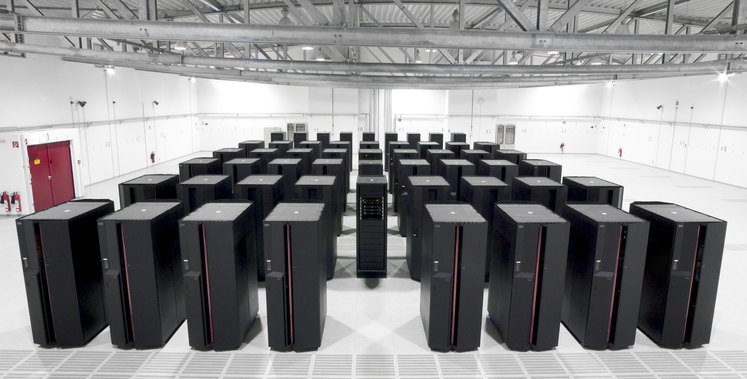
\includegraphics[width=\textwidth]{supercomputer.png}
  \begin{itemize}
  \item Code needs to be ready to run ASAP.
  \item Test as much as possible before hand.
  \end{itemize}
\end{frame}

\begin{frame}[fragile]
  \frametitle{Code Attractiveness}
  \vspace{1cm}
  \epigraph{``Code without tests is broken by design.''}{--- \textup{Jacob Kaplan-Moss}, Django documentation}
\end{frame}

\begin{frame}
  \frametitle{Working in Teams}
  \begin{tikzpicture}[
      >=stealth,
      node distance=2.5cm,
      database/.style={
        cylinder,
        cylinder uses custom fill,
        cylinder body fill=Base09,
        cylinder end fill=Base0A,
        shape border rotate=90,
        aspect=0.25,
        draw,
        text=Base06
      },
      user/.style={
        circle,
        fill=Base0D,
        text=Base06
      },
      overlay,
      shift={(5,-0.5)}
    ]
    \node[database] (db) at (0,0) {DB};
    \node[user,right of=db] (u1) {User};
    \node[user,below of=db] (u2) {User};
    \node[user,above of=db] (u3) {User};
    \node[user,left of=db]  (u4) {User};

    \draw[->] (db) -- (u1);
    \draw[->] (db) -- (u2);
    \draw[->] (db) -- (u3);
    \draw[->] (db) -- (u4);
  \end{tikzpicture}
\end{frame}
